\documentclass[a4paper,12pt]{article}

\usepackage[14pt]{extsizes}
\usepackage{cmap}					% поиск в PDF
\usepackage{mathtext} 				% русские буквы в формулах
\usepackage[T2A]{fontenc}			% кодировка
\usepackage[utf8]{inputenc}			% кодировка исходного текста
\usepackage[english,russian]{babel}	% локализация и переносы
\usepackage{graphicx}
\usepackage{geometry}
\usepackage{amsmath}
\usepackage{multirow}
\usepackage[table]{xcolor}
\setlength\extrarowheight{2pt}


\geometry{verbose, a4paper, tmargin=2cm, bmargin=2cm, lmargin=3cm, rmargin=2cm}
\author{Vysotsky Maxim}
\title{Отчёт}
\date{2022}

\begin{document}
	\begin{titlepage}
		\begin{center}
			{Министерство науки и высшего образования Российской Федерации
				НОВОСИБИРСКИЙ НАЦИОНАЛЬНЫЙ ИССЛЕДОВАТЕЛЬСКИЙ
				ГОСУДАРСТВЕННЫЙ УНИВЕРСИТЕТ (НГУ)}
		\end{center}
		\begin{center}
			{Физический факультет}
		\end{center}
		
		
		\vspace{8cm}
		{
			\begin{center}
				{\bf Лабораторная работа №7}\\
				Измерение ускорения свободного падения
			\end{center}
		}
		\vspace{2cm}
		\begin{flushright}
			{Руководитель:\\ Старший преподаватель\\
				Яцких А. А.\\
				Работу выполнил:\\
				Высоцкий М. Ю.\\
				\vspace{0.2cm}
				гр. 24301}
		\end{flushright}
		\vspace{3cm}
		\begin{center}
			Новосибирск, 2024
		\end{center}
	\end{titlepage}

\section{Теоретическое введение}
Цель работы: определение величины ускорения свободного падения баллистическим методом 

\begin{figure}[h!]
	\begin{center}
		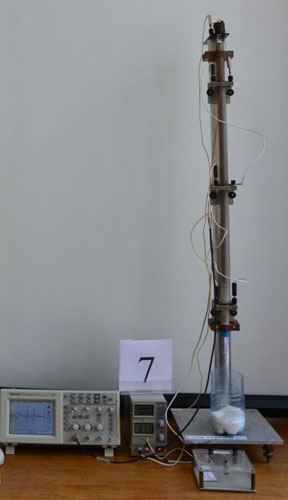
\includegraphics[scale=0.8]{ust.jpg}
	\end{center}
	\caption{Фотография установки.}
\end{figure}

Рабочая формула:
\begin{equation}
    S = gT \longrightarrow g = \frac{S}{T}
\end{equation}

\begin{equation}
    T = g\frac{t_1*t_2}{2} * \frac{t_1+t_2}{t_1-t_2}
\end{equation}

\clearpage
\section{Ход работы}
  
\begin{center}
    
\begin{tabular}{|l|l|l|l|l|}
\hline
S, см &t1, мс & t2, мс & T, мс^2 & g, м/с^2\\ \hline
\multirow{5}{*}{35}       & 143                        & 97                         & 36185,22                                     & 9,67                                          \\
                          & 129                        & 92                         & 35443,62                                     & 9,87                                          \\
                          & 134                        & 95                         & 37373,97                                     & 9,36                                          \\
                          & 138                        & 97                         & 38362,32                                     & 9,12                                          \\
                          & 140                        & 98                         & 38873,33                                     & 9,00                                          \\ \hline
\multirow{5}{*}{30}       & 108                        & 83                         & 34242,48                                     & 8,76                                          \\
                          & 102                        & 81                         & 35998,71                                     & 8,33                                          \\
                          & 107                        & 84                         & 37319,74                                     & 8,04                                          \\
                          & 109                        & 82                         & 31614,04                                     & 9,49                                          \\
                          & 105                        & 82                         & 35001,52                                     & 8,57                                          \\ \hline
\multirow{5}{*}{25}       & 83                         & 70                         & 34189,62                                     & 7,31                                          \\
                          & 82                         & 65                         & 23044,41                                     & 10,85                                         \\
                          & 84                         & 71                         & 35554,62                                     & 7,03                                          \\
                          & 94                         & 75                         & 31353,95                                     & 7,97                                          \\
                          & 84                         & 70                         & 32340,00                                     & 7,73                                          \\ \hline
\multirow{5}{*}{20}       & 63,6                       & 58,4                       & 43570,89                                     & 4,59                                          \\
                          & 62,4                       & 54,4                       & 24780,29                                     & 8,07                                          \\
                          & 62,8                       & 54,4                       & 23832,90                                     & 8,39                                          \\
                          & 61,2                       & 53,6                       & 24775,05                                     & 8,07                                          \\
                          & 62,8                       & 55,2                       & 26911,45                                     & 7,43                                          \\ \hline
\multirow{5}{*}{15}       & 42                         & 38                         & 15960,00                                     & 9,40                                          \\
                          & 42,4                       & 38,8                       & 18553,30                                     & 8,08                                          \\
                          & 42,8                       & 38,8                       & 16938,53                                     & 8,86                                          \\
                          & 42                         & 39,6                       & 28274,40                                     & 5,31                                          \\
                          & 43,6                       & 39,6                       & 17956,22                                     & 8,35                                          \\ \hline
\multirow{5}{*}{10}       & 28                         & 26                         & 9828,00                                      & 10,18                                         \\
                          & 28,4                       & 26                         & 8368,53                                      & 11,95                                         \\
                          & 27,6                       & 25,6                       & 9397,25                                      & 10,64                                         \\
                          & 27,6                       & 25,6                       & 9397,25                                      & 10,64                                         \\
                          & 28,4                       & 26,4                       & 10271,71                                     & 9,74         
                          \\ \hline
\end{tabular}
\end{center}
\clearpage
Для серий получились значения:
$$ g_1 = 9,41 \pm 0,16$$
$$ g_2 = 8,64 \pm 0,24$$
$$ g_3 = 8,18 \pm 0,69$$
$$ g_4 = 7,31 \pm 0,70$$
$$ g_5 = 8,00 \pm 0,71$$
$$ g_6 = 10,63 \pm0,37$$


\end{document}